\documentclass[letterpaper,11pt,oneside,reqno]{article}

%%%%%%%%%%%%%%%%%%%%%%%%%%%%%%%%%%%%%%%%%%%%%%%%%%%%%%%%%%%%

\usepackage[pdftex,backref=page,colorlinks=true,linkcolor=blue,citecolor=red]{hyperref}
\usepackage[alphabetic,nobysame]{amsrefs}

%%%%%%%%%%%%%%%%%%%%%%%%%%%%%%%%%%%%%%%%%%%%%%%%%%%%%%%%%%%%
%main packages
\usepackage{amsmath,amssymb,amsthm,amsfonts,mathtools}
\usepackage{graphicx,color}
\usepackage{upgreek}
\usepackage[mathscr]{euscript}

%equations
\allowdisplaybreaks
\numberwithin{equation}{section}

%tikz
\usepackage{tikz}
\usetikzlibrary{shapes,arrows,positioning,decorations.markings}

%conveniences
\usepackage{array}
\usepackage{adjustbox}
\usepackage{cleveref}
\usepackage{enumerate}
\usepackage{datetime}

%paper geometry
\usepackage[DIV=12]{typearea}

%%%%%%%%%%%%%%%%%%%%%%%%%%%%%%%%%%%%%%%%%%%%%%%%%%%%%%%%%%%%
%draft-specific
\synctex=1
% \usepackage{refcheck,comment}

%%%%%%%%%%%%%%%%%%%%%%%%%%%%%%%%%%%%%%%%%%%%%%%%%%%%%%%%%%%%
%this paper specific
\newcommand{\ssp}{\hspace{1pt}}

%%%%%%%%%%%%%%%%%%%%%%%%%%%%%%%%%%%%%%%%%%%%%%%%%%%%%%%%%%%%
\newtheorem{proposition}{Proposition}[section]
\newtheorem{lemma}[proposition]{Lemma}
\newtheorem{corollary}[proposition]{Corollary}
\newtheorem{theorem}[proposition]{Theorem}
%%%%%%%%%%%%%%%%%%%%%%%%%%%%%%%%%%%%%%%%%%%%%%%%%%%%%%%%%%%%
\theoremstyle{definition}
\newtheorem{definition}[proposition]{Definition}
\newtheorem{remark}[proposition]{Remark}
%%%%%%%%%%%%%%%%%%%%%%%%%%%%%%%%%%%%%%%%%%%%%%%%%%%%%%%%%%%%

\newenvironment{lnotes}{\section*{Notes for the lecturer}}{}

% \excludecomment{lnotes}

\begin{document}
\title{Lectures on Random Matrices
(Spring 2025)
\\Lecture 6: Double contour integral kernel. Steepest descent and local statistics}

\date{February 12, 2025\footnote{\href{https://lpetrov.cc/rmt25/}{\texttt{Course webpage}}
$\bullet$ \href{https://lpetrov.cc/simulations/model/random-matrices/}{\texttt{Live simulations}}
$\bullet$ \href{https://lpetrov.cc/rmt25/rmt25-notes/rmt2025-l06.tex}{\texttt{TeX Source}}
$\bullet$
Updated at \currenttime, \today}}

\author{Leonid Petrov}

\maketitle

\begin{lnotes}
	1. GUE det structure

	2. Formulate Cauchy--Binet and Andreief

	3. Recall that $\rho_n=P_n$ and it is
	$\left( \det[\psi_i(x_j)]_{n\times n} \right)^2$, then reproduce the proofs here.
\end{lnotes}

\section{Recap: Determinantal structure of the GUE}

Last time, we proved the following result:
\begin{theorem}
\label{thm:determinantal_GUE}
The GUE correlation functions are given by
\[
\rho_k(x_1,\dots,x_k)=\det\Bigl[K_n(x_i,x_j)\Bigr]_{i,j=1}^k,
\]
with the correlation kernel
\[
K_n(x,y)=\sum_{j=0}^{n-1}\psi_j(x)\psi_j(y).
\]
Here
\begin{equation*}
	\psi_j(x)=\frac{1}{\sqrt{h_j}}\ssp p_j(x)\,e^{-x^2/4},
\end{equation*}
where \(p_j(x)\) are the monic Hermite polynomials, and \(h_j\) are the normalization constants so that
$\psi_j(x)$ are orthonormal in $L^2(\mathbb{R})$.
\end{theorem}

For this theorem, we need Cauchy--Binet summation formula
and Andreief identity (which is essentially the same as Cauchy--Binet, but when summation is
replaced by integration). Having these, we can write
\begin{align*}
	\rho_k(x_1,\dots,x_k)&=\frac{n!}{(n-k)!}\int_{\mathbb{R}^{n-k}} p(x_1,\dots,x_n) \,dx_{k+1}\cdots dx_n
	\\
	&=
	\frac{1}{(n-k)!\,\widehat{Z}_{n,2}}
	\sum_{\substack{\sigma,\tau\in S_n\\
	\sigma(k+1)=\tau(k+1),\ldots,\sigma(n)=\tau(n) }} \operatorname{sgn}(\sigma)\operatorname{sgn}(\tau)
	\prod_{i=1}^k \psi_{\sigma(i)-1}(x_i)\psi_{\tau(i)-1}(x_i)
	\\
	&=
	\mathrm{const}_n\sum_{I\subseteq [n],\,|I|=k}
	\sum_{\sigma',\tau'\in S(I)}
	\operatorname{sgn}(\sigma')\operatorname{sgn}(\tau')
	\prod_{i=1}^k \psi_{\sigma'(i)-1}(x_i)\psi_{\tau'(i)-1}(x_i)
	\\
	&=
	\mathrm{const}_n\sum_{I\subseteq [n],\,|I|=k}
	\det\left[ \psi_{i_\alpha}(x_j) \right]_{\alpha,j=1}^k
	\det\left[ \psi_{i_\alpha}(x_j) \right]_{\alpha,j=1}^k,
\end{align*}
where \(I=\{i_1,\ldots,i_k\}\) is a subset of \([n]\) of size \(k\), and \(S(I)\) is the set of permutations of \(I\).
The last sum of products of two determinants is
written by the Cauchy--Binet formula as
\begin{equation*}
	\mathrm{const}_n\cdot \det\left[ \sum_{j=0}^{n-1}\psi_j(x_\alpha)\psi_j(x_\beta) \right]_{\alpha,\beta=1}^k,
\end{equation*}
and finally the constant is equal to $1$ by Andreief identity.


%%%%%%%%%%%%%%%%%%%%%%%%%%%%%%%%%%%%%%%%%%%%%%%%%%%%%%%%%%%%
\section{Double Contour Integral Representation for the GUE Kernel}
\label{sec:double-contour}

\subsection{One contour integral representation for Hermite polynomials}

Recall that the GUE kernel is defined by
\[
K_N(x,y)=\sum_{n=0}^{N-1}\psi_n(x)\psi_n(y),
\]
with the orthonormal functions
\[
\psi_n(x)=\frac{1}{\sqrt{h_n}}\,p_n(x)\,e^{-x^2/4},
\]
where the (monic, probabilists') Hermite polynomials are given by
\begin{equation}
\label{eq:hermite_def}
	p_n(x)=(-1)^n e^{x^2/2}\frac{d^n}{dx^n}\,e^{-x^2/2}.
\end{equation}
Note that the monic Hermite polynomials are uniquely defined by the
orthogonality property. We are not proving \eqref{eq:hermite_def} here,
it is an exercise.
\begin{lemma}[Generator function for Hermite polynomials]
	\label{lem:hermite_gen}
	We have
	\[
		\exp\Bigl(xt-\frac{t^2}{2}\Bigr)=\sum_{n\ge0}p_n(x)\frac{t^n}{n!}.
	\]
	The series converges for all \(t\) since the left-hand side is an entire function of \(t\).
\end{lemma}
\begin{proof}
Write the generating function as
\[
	\sum_{n\ge0}p_n(x)\frac{t^n}{n!}
	=\sum_{n\ge0}\frac{(-1)^n t^n}{n!}\,e^{x^2/2}\frac{d^n}{dx^n}\,e^{-x^2/2}.
\]
Since the factor \(e^{x^2/2}\) does not depend on \(n\), we can factor it out:
\[
	\sum_{n\ge0}p_n(x)\frac{t^n}{n!}= e^{x^2/2}\sum_{n\ge0}\frac{(-t)^n}{n!}\frac{d^n}{dx^n}\,e^{-x^2/2}.
\]
Now, recall Taylor's theorem: for any analytic function \(f\) we have
\[
	f(x-t)=\sum_{n\ge0}\frac{(-t)^n}{n!}f^{(n)}(x).
\]
Applying this with \(f(x)=e^{-x^2/2}\), we deduce that
\[
	\sum_{n\ge0}\frac{(-t)^n}{n!}\frac{d^n}{dx^n}\,e^{-x^2/2}= e^{-(x-t)^2/2}.
\]
Thus, our generating function becomes
\[
	\sum_{n\ge0}p_n(x)\frac{t^n}{n!} = e^{x^2/2}\, e^{-(x-t)^2/2},
\]
as desired.
\end{proof}


By Cauchy's integral formula we can write using \Cref{lem:hermite_gen}:
\begin{equation}
\label{eq:pn-formula}
p_n(x)=\frac{n!}{2\pi i}\oint_C\frac{\exp\Bigl(xt-\frac{t^2}{2}\Bigr)}{t^{n+1}}\,dt,
\end{equation}
where the contour \(C\) is a simple closed curve encircling the origin.
Indeed, here we use the complex analysis property
\begin{equation*}
	\frac{1}{2\pi i}\oint_C \frac{1}{z^{k+1}}\ssp dz=\begin{cases}
		1,&\text{ if }k=0,\\
		0,&\text{ if }k\neq0,
	\end{cases}
\end{equation*}
so \eqref{eq:pn-formula} is simply a complex analysis version of the
operation of extracting the coefficient of \(t^n\) in the Taylor expansion.

Therefore,
\begin{equation*}
	\psi_n(x)=\frac{1}{\sqrt{h_n}}\,p_n(x)\,e^{-x^2/4}=
	\frac{e^{-x^2/4}}{\sqrt{h_n}}\frac{n!}{2\pi i}\oint_C\frac{\exp\Bigl(xt-\frac{t^2}{2}\Bigr)}{t^{n+1}}\,dt.
\end{equation*}

\subsection{Another contour integral representation for Hermite polynomials}

We start with the Fourier transform identity
\[
\int_{-\infty}^{\infty} \exp\Bigl(-\frac{t^2}{2} + i\,t\,x\Bigr)\,dt
=\sqrt{2\pi}\,e^{-x^2/2}.
\]
Differentiating both sides \(n\) times with respect to \(x\) yields
\[
\frac{d^n}{dx^n}\Bigl(e^{-x^2/2}\Bigr)
=\frac{1}{\sqrt{2\pi}}\int_{-\infty}^{\infty} (i\,t)^n\,e^{-t^2/2+ i\,t\,x}\,dt.
\]
Recalling the definition
\[
p_n(x)=(-1)^n\,e^{x^2/2}\,\frac{d^n}{dx^n}\Bigl(e^{-x^2/2}\Bigr),
\]
we obtain
\[
p_n(x)=\frac{(-1)^n\,e^{x^2/2}}{\sqrt{2\pi}}\int_{-\infty}^{\infty}(i\,t)^n\,e^{-t^2/2+ i\,t\,x}\,dt.
\]

Next, perform the change of variable
\[
s=i\,t,\quad\text{so that}\quad t=-i\,s,\quad dt=-i\,ds.
\]
Under this substitution the factors transform as follows:
\[
(i\,t)^n = s^n,
\]
and the exponent becomes
\[
-\frac{t^2}{2}+ i\,t\,x
= -\frac{(-i\,s)^2}{2}+ i\,(-i\,s)\,x
= \frac{s^2}{2}+ s\,x.
\]
Thus, the integral transforms into
\[
\int_{-\infty}^{\infty}(i\,t)^n\,e^{-t^2/2+ i\,t\,x}\,dt
= -i \int_{-i\infty}^{i\infty} s^n\,e^{s^2/2+ s\,x}\,ds.
\]
Substituting back we have
\[
p_n(x)=\frac{(-1)^n\,e^{x^2/2}}{\sqrt{2\pi}}\;(-i)
\int_{-i\infty}^{i\infty} s^n\,e^{s^2/2+ s\,x}\,ds.
\]
That is,
\[
p_n(x)=\frac{i\,(-1)^{n+1}\,e^{x^2/2}}{\sqrt{2\pi}}
\int_{-i\infty}^{i\infty} s^n\,e^{s^2/2+ s\,x}\,ds.
\]
Finally, change the sign of $s$, and we get:
\[
p_n(x)=\frac{i\,e^{x^2/2}}{\sqrt{2\pi}}
\int_{-i\infty}^{i\infty} s^n\,e^{s^2/2- s\,x}\,ds.
\]
Therefore,
\[
\psi_n(x)=\frac{i\,e^{x^2/4}}{\sqrt{2\pi\,h_n}}
\int_{-i\infty}^{i\infty} s^n\,e^{s^2/2- s\,x}\,ds.
\]

\subsection{Normalization of Hermite polynomials}

\begin{lemma}
	\label{lem:hermite_norm}
	We have
	\begin{equation*}
		h_n=\int_{-\infty}^{\infty} p_n(x)^2\,e^{-x^2/2}\,dx=n!\sqrt{2\pi}.
	\end{equation*}
\end{lemma}
\begin{proof}
Multiply the generating function
\[
	\exp\Bigl(xt-\frac{t^2}{2}\Bigr)=\sum_{n\ge0}p_n(x)\frac{t^n}{n!}
\]
with a second copy (with parameter \(s\)):
\[
	\exp\Bigl(xs-\frac{s^2}{2}\Bigr)=\sum_{m\ge0}p_m(x)\frac{s^m}{m!}.
\]
Then,
\[
	\exp\Bigl(xt-\frac{t^2}{2}\Bigr)\exp\Bigl(xs-\frac{s^2}{2}\Bigr)
	=\sum_{n,m\ge0}p_n(x)p_m(x)\frac{t^n s^m}{n!m!}.
\]
Integrate both sides against \(e^{-x^2/2}\,dx\). Using the orthogonality
\[
	\int_{-\infty}^{\infty}p_n(x)p_m(x)e^{-x^2/2}dx=h_n\delta_{nm},
\]
the right-hand side becomes
\[
	\sum_{n\ge0}\frac{h_n}{(n!)^2}(ts)^n.
\]
On the left-hand side, we have
\[
	\int_{-\infty}^{\infty}e^{-x^2/2}\exp\Bigl(x(t+s)-\frac{t^2+s^2}{2}\Bigr)dx.
\]
Completing the square in \(x\) or recalling the standard Gaussian integral yields
\[
	\sqrt{2\pi}\exp\Bigl(\frac{(t+s)^2-(t^2+s^2)}{2}\Bigr)
	=\sqrt{2\pi}\exp(ts).
\]
Thus, we obtain
\[
	\sqrt{2\pi}\exp(ts)=\sum_{n\ge0}\frac{h_n}{(n!)^2}(ts)^n.
\]
Expanding the left side as
\[
	\sqrt{2\pi}\sum_{n\ge0}\frac{(ts)^n}{n!},
\]
and comparing coefficients, we conclude that
\[
	\frac{h_n}{(n!)^2}=\frac{\sqrt{2\pi}}{n!}\quad\Longrightarrow\quad h_n=n!\sqrt{2\pi}.
\]
This completes the proof.
\end{proof}

\subsection{Double contour integral representation for the GUE kernel}

We can sum up the kernel (essentially, this is
another proof of the Christoffel--Darboux formula):
\begin{equation}\begin{split}
	K_n(x,y)&=
	\sum_{k=0}^{n-1}\psi_k(x)\psi_k(y)
	\\&=
	\frac{e^{\frac{x^2-y^2}{4}}}{(2\pi)^2}
	\oint_C dt\int_{-i\infty}^{i\infty}ds\ssp
	\exp\left\{ -\frac{t^2}{2}+xt+\frac{s^2}{2}-ys \right\}
	\underbrace{\sum_{k=0}^{n-1}
	s^k t^{-k-1}}_{\frac{1-(s/t)^n}{t-s}}.
\end{split}\label{eq:K_n_sum}\end{equation}
Here we used the two contour integral representations for Hermite polynomials,
and the explicit norm (\Cref{lem:hermite_norm}).
At this point, the $t$ contour is a small circle around $0$, and
the $s$ contour is a vertical line in the complex plane.
Their mutual position can be arbitrary at this point --- the $s$ contour
goes along the imaginary line.
Indeed, the fraction
$\frac{1-(s/t)^n}{t-s}$ does not have a singularity at $s=t$ due to the
cancellation.

Let us now move the $s$ contour to be to the left of the $t$ contour,
as in \Cref{fig:contours}.
On the new contours, we have $|s|>|t|$.
Now we can add the summands $s^k t^{-k-1}$ 
for all $k\le -1$
into the sum in
\eqref{eq:K_n_sum}. 
Indeed, for $|s|>|t|$, the series in $k$ converges, while the 
summand $s^kt^{-k-1}$ has zero residue at $0$ and thus adding the 
summands does not change the value of the integral.

\begin{figure}[htpb]
	\centering
	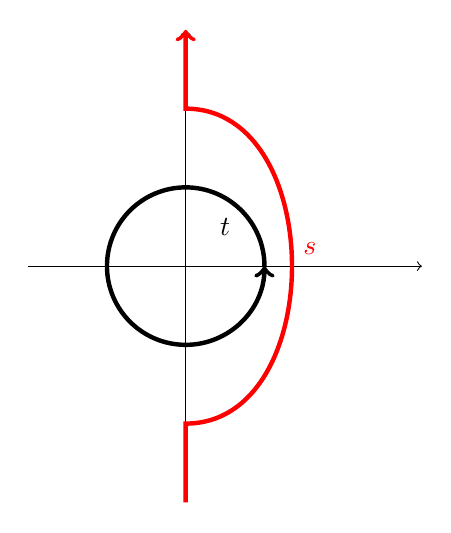
\begin{tikzpicture}[scale=1]
		% Draw coordinate axes
		\draw[->] (-2,0) -- (3,0);
		\draw[->] (0,-3) -- (0,3);

		% t contour: unit circle, counterclockwise
		\draw[ultra thick,->] (1,0) arc (0:360:1);
		% Place the t label near the contour (at 45° outside the circle)
		\coordinate (TLabel) at (.5,.5);
		\node at (TLabel) {\(t\)};

		% s contour: vertical line (imaginary axis) with a detour near the origin
		% It starts at (0,-3), goes vertically to (0,-2), then detours to (0,2)
		% via a Bézier curve (pushed to the right), and finally resumes vertically to (0,3).
		\draw[ultra thick,->,red]
			(0,-3)
			-- (0,-2)
			.. controls (1.8,-2) and (1.8,2) .. node[midway, above right] {\(s\)} (0,2)
			-- (0,3);
	\end{tikzpicture}
	\caption{Integration contours for the GUE kernel \eqref{eq:K_n_GUE_kernel}.}
	\label{fig:contours}
\end{figure}

With this extension of the sum, formula \eqref{eq:K_n_sum} becomes
\begin{equation}
	\label{eq:K_n_GUE_kernel}
	K_n(x,y)=\frac{e^{(y^2-x^2)/4}}{(2\pi)^2}
	\oint_C dt\int_{-i\infty}^{i\infty}ds\ssp
	\frac{\exp\left\{ \frac{s^2}{2}-sy-\frac{t^2}{2}+tx \right\}}{s-t}\left( \frac{s}{t} \right)^n\ssp .
\end{equation}




\subsection{Extensions}

Many other versions of the GUE / unitary invariant ensembles admit determinantal structure:
\begin{enumerate}
	\item The GUE corners process \cite{johansson2006eigenvalues}
    \item The Dyson Brownian motion (e.g., add a GUE to a diagonal matrix)
			\cite{nagao1998multilevel}
		\item GUE corners plus a fixed matrix \cite{Ferrari2014PerturbedGUE}
    \item Corners invariant ensembles with fixed eigenvalues $UDU^\dagger$, where $D$ is a fixed diagonal matrix and $U$ is Haar distributed
			on the unitary group \cite{Metcalfe2011GT}
	\end{enumerate}

%%%%%%%%%%%%%%%%%%%%%%%%%%%%%%%%%%%%%%%%%%%%%%%%%%%%%%%%%%%%





















\appendix
\setcounter{section}{5}

\section{Problems (due 2025-03-12)}





\bibliographystyle{alpha}
\bibliography{bib}


\medskip

\textsc{L. Petrov, University of Virginia, Department of Mathematics, 141 Cabell Drive, Kerchof Hall, P.O. Box 400137, Charlottesville, VA 22904, USA}

E-mail: \texttt{lenia.petrov@gmail.com}


\end{document}
